%%%%%%%%%%%%%%%%%%%%%%%%%%%%%%%%%%%%%%%%%
% Memo
% LaTeX Template
% Version 1.0 (30/12/13)
%
% This template has been downloaded from:
% http://www.LaTeXTemplates.com
%
% Original author:
% Rob Oakes (http://www.oak-tree.us) with modifications by:
% Vel (vel@latextemplates.com)
%
% License:
% CC BY-NC-SA 3.0 (http://creativecommons.org/licenses/by-nc-sa/3.0/)
%
%%%%%%%%%%%%%%%%%%%%%%%%%%%%%%%%%%%%%%%%%

\documentclass[letterpaper,11pt]{texMemo} % Set the paper size (letterpaper, a4paper, etc) and font size (10pt, 11pt or 12pt)

\usepackage{parskip} % Adds spacing between paragraphs
\setlength{\parindent}{15pt} % Indent paragraphs

%----------------------------------------------------------------------------------------
%	MEMO INFORMATION
%----------------------------------------------------------------------------------------

\memoto{Dr. Randy C. Hoover} % Recipient(s)

\memofrom{Sharif Anani} % Sender(s)

\memosubject{Template Matching - ``Where's Waldo''} % Memo subject

\memodate{Thursday, October 22, 2015} % Date, set to \today for automatically printing todays date

\logo{
\includegraphics[width=0.1\textwidth]{logo.png}} % Institution logo at the top right of the memo, comment out this line for no logo

%----------------------------------------------------------------------------------------

\begin{document}

\maketitle % Print the memo header information

%----------------------------------------------------------------------------------------
%	MEMO CONTENT
%----------------------------------------------------------------------------------------

\section{Assignment Summary}
The assignment requires that the student writes a \textsc{Matlab} function that does correlation between a kernel image and a scene image. The purpose of this function is to be used for template matching: i.e. finding a template in the image.

\section{Mathematical Background}
The mathematics behind this simple method of template matching are very simple. Correlating a patch (kernel) with the image (scene) and finding the area where the result is maximum. The maximum result is the result with the best match.\\
Problems with this method is that due to different sizes between the kernel and scene sizes, both have different mean and standard deviation, which can result in inconclusve results.\\
The classic correlation equation is as follows:\\
\begin{equation}
r(i,j) = \sum_{n=1}^{N} \sum_{m=1}^{M} A(m,n)B(m-i,n-j)
\end{equation}\\

To solve this problem, we can use a normalized cross-correllation. In normalized cross-correlation, each set's mean is subtracted from it, and each set is divided by its own standard deviation. This way both samples have a mean of zero and a standard deviation of 1. The equation of normalized cross-correlation is as follows:\\

\begin{equation}
r(i,j) = \sum_{n=1}^{N} \sum_{m=1}^{M} \frac{A(m,n)-\bar{A}}{\sigma_{A}}\frac{B(m-i,n-j)-\bar{B}}{\sigma_{B}}
\end{equation}\\

\section{Details About The Method}
Before executing the method, both images are conditioned to get better results. This conditioning consists of converting both images into the ``L a b'' color space, where the L channel is for Luminance, i.e., it results in a grayscale image, and the a \& b channels are color channels.\\
The method is executed on all three channels which are then restacked into one image matrix.\\
The results shown are only from the L channel, however the function does the correlation using all three channels.
\section{Results}
The following images show the kernel, the scene, the result, and the final result of the scene with the match point circled.
\begin{figure}[!h]
	\centering
		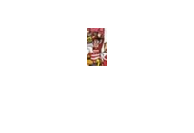
\includegraphics{kernel.png}
	\caption{Kernel}
	\label{fig:kernel}
\end{figure}
\\
\begin{figure}[!h]
	\centering
		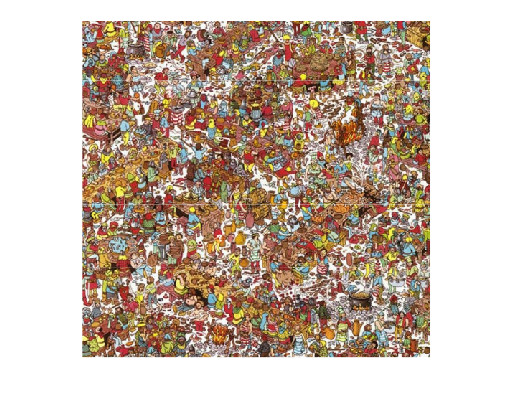
\includegraphics[width=0.50\textwidth]{scene.png}
	\caption{Scene}
	\label{fig:scene}
\end{figure}
\\
\begin{figure}[!h]
	\centering
		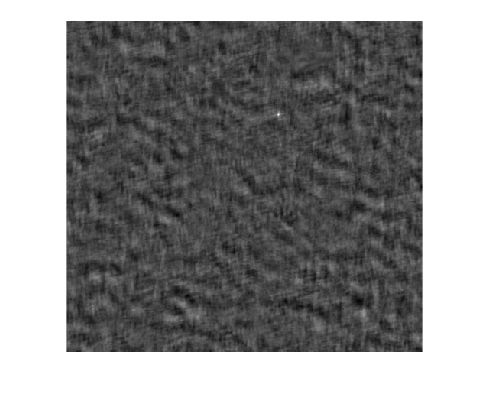
\includegraphics{result.png}
	\caption{result}
	\label{fig:result}
\end{figure}
\\
\begin{figure}
	\centering
		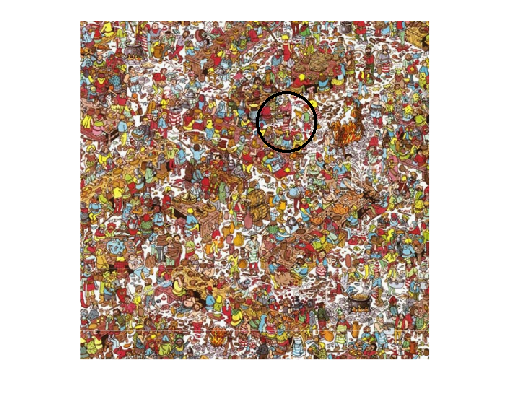
\includegraphics{final.png}
	\caption{Final Result}
	\label{fig:final}
\end{figure}


%----------------------------------------------------------------------------------------

\end{document}